
\section{Evaluating Depth-Based Tiebreaking}
\label{sec:depth-based-evaluation}
We evaluated our depth-based diversifying tiebreaking strategies against standard
tiebreaking strategies.
In addition to the 35 IPC benchmark domains with 1104 instances used in
the previous set of experiments, we used 28 zerocost domains with 620
instances.

\subsection{Evaluating Depth-Based Tiebreaking with $h$-tiebreaking}

We compared the performance of standard tiebreaking methods $[f,h,\fifo]$,
$[f,h,\lifo]$ to $[f,h,\depth,\fifo]$ and
$[f,h,\depth,\lifo]$.  These all use $h$ as the first-level
tiebreaking and either \fifo or \lifo as the last-resort tiebreaking.

First two experiments are conducted on \textbf{1104 standard IPC
benchmark instances}, and the latter two experiments are conducted on
\textbf{620 zerocost instances}.  Each experiment uses either \lmcut
heuristics or \mands heuristics.  For \mands heuristics, we used the
settings recommended by Fast Downward website (bisimulation-based shrink
strategy, DFP merge strategy and exact label reduction).

We first show the summary results of these experiments.
Overall, depth-based tiebreaking tends to show larger coverages than the
standard tiebreaking strategies. In the following, we describe the
details of each experiments.

\begin{table}[htb]
 {
 \centering
\begin{tabular}{|*{5}{c|}}
\hline
 & \multicolumn{4}{|c|}{\lmcut Coverages (\# problems solved)}\\
\hline                                    
 Domain               &  $[f,h,\fifo]$ &  $[f,h,\lifo]$ &  $[f,h,\depth,\fifo]$ &  $[f,h,\depth,\lifo]$ \\ \hline
 IPC,\lmcut(1104)     &558             &565             &\textbf{570.6\spm{}1.5}      &560.0\spm{}0.9               \\ 
 IPC,\mands(1104)     &479             &\textbf{488}    &484.0\spm{}0.0               &481.4\spm{}1.4               \\ \hline
 Zerocost,\lmcut(620) &256             &279             &\textbf{287.2\spm{}2.4}      &280.2\spm{}4.2               \\ 
 Zerocost,\mands(620) &276             &290             &\textbf{310.2\spm{}2.1}      &303.2\spm{}1.7               \\ \hline
\end{tabular}
 \caption{
 Summary Results: Coverage comparison (the number of instances solved in 5min, 2GB, \lmcut/\mands
 heuristics) between standard tiebreaking and depth-based tiebreaking ($\depth$). }
 \label{tbl:lmcut-ipc-full}
 }
\end{table}

\reftbl{tbl:lmcut-ipc-full} shows the number of \textbf{1104 standard
IPC benchmark instances} solved by \lmcut heuristics with various
tiebreaking strategies, under 5min, 2GB experiments. We highlight the
best results when the difference between the maximum and the mininum
coverage exceeds 2.  Depth-based tiebreaking ($\depth$) shows
impressive results on Openstacks and Cybersec domains because these
domains contain many instances of zero-cost edges and the final plateau
$\plateau{f,h}$ is huge (See \refig{fig:plateau}).  Most other instances
are unaffected by depth-based tiebreaking.  Thus, our method offers a
better performance in the domains of interest for free, i.e. without
losing performance in other domains.

\begin{table}[htbp]
 {
 \centering
 \begin{tabular}{|*{5}{c|}}
\hline
 & \multicolumn{4}{|c|}{\lmcut Coverages (\# problems solved)}\\
\hline                                    
 Domain                                 &  $[f,h,\fifo]$ &  $[f,h,\lifo]$ &  $[f,h,\brackets{d},\fifo]$       &  $[f,h,\brackets{d},\lifo]$        \\ \hline                                    
 sum(1104)                              &558             &565             &\textbf{570.6\spm{}1.5} &560.0\spm{}0.9         \\ \hline                                    
 {\relsize{-1}airport(50)}              &\textbf{27}     &26              &25.9\spm{}0.5           &21.0\spm{}0.0          \\
 {\relsize{-1}barman-opt11(20)}         &0               &0               &0.0\spm{}0.0            &0.0\spm{}0.0           \\
 {\relsize{-1}blocks(35)}               &28              &28              &28.0\spm{}0.0           &27.0\spm{}0.0          \\
 {\relsize{-1}cybersec(19)}             &2               &3               &\textbf{9.6\spm{}1.1}   &7.8\spm{}0.7           \\
 {\relsize{-1}depot(22)}                &6               &6               &6.0\spm{}0.0            &6.0\spm{}0.0           \\
 {\relsize{-1}driverlog(20)}            &13              &13              &13.0\spm{}0.0           &13.0\spm{}0.0          \\
 {\relsize{-1}elevators-opt11(20)}      &15              &15              &15.0\spm{}0.0           &14.8\spm{}0.4          \\
 {\relsize{-1}floortile-opt11(20)}      &6               &6               &6.0\spm{}0.0            &6.0\spm{}0.0           \\
 {\relsize{-1}freecell(80)}             &9               &9               &9.0\spm{}0.0            &9.0\spm{}0.0           \\
 {\relsize{-1}grid(5)}                  &1               &1               &1.0\spm{}0.0            &1.0\spm{}0.0           \\
 {\relsize{-1}gripper(20)}              &6               &6               &6.0\spm{}0.0            &6.0\spm{}0.0           \\
 {\relsize{-1}hanoi(30)}                &12              &12              &12.0\spm{}0.0           &12.0\spm{}0.0          \\
 {\relsize{-1}logistics00(28)}          &\textbf{20}     &\textbf{20}     &\textbf{20.0\spm{}0.0}  &\textbf{20.0\spm{}0.0} \\
 {\relsize{-1}miconic(150)}             &\textbf{140}    &\textbf{140}    &\textbf{140.0\spm{}0.0} &135.6\spm{}0.5         \\
 {\relsize{-1}mprime(35)}               &21              &21              &20.9\spm{}0.3           &21.0\spm{}0.0          \\
 {\relsize{-1}mystery(30)}              &15              &16              &15.0\spm{}0.0           &15.8\spm{}0.4          \\
 {\relsize{-1}nomystery-opt11(20)}      &14              &14              &14.0\spm{}0.0           &13.8\spm{}0.4          \\
 {\relsize{-1}openstacks-opt11(20)}     &11              &\textbf{18}     &\textbf{18.0\spm{}0.0}  &\textbf{18.0\spm{}0.0} \\
 {\relsize{-1}parcprinter-opt11(20)}    &13              &13              &13.0\spm{}0.0           &13.0\spm{}0.0          \\
 {\relsize{-1}parking-opt11(20)}        &1               &1               &1.0\spm{}0.0            &1.0\spm{}0.0           \\
 {\relsize{-1}pathways(30)}             &5               &5               &5.0\spm{}0.0            &5.0\spm{}0.0           \\
 {\relsize{-1}pegsol-opt11(20)}         &17              &17              &17.0\spm{}0.0           &17.0\spm{}0.0          \\
 {\relsize{-1}pipesworld-notankage(50)} &15              &14              &14.2\spm{}0.4           &14.2\spm{}0.4          \\
 {\relsize{-1}pipesworld-tankage(50)}   &8               &8               &8.0\spm{}0.0            &8.0\spm{}0.0           \\
 {\relsize{-1}psr-small(50)}            &48              &48              &48.0\spm{}0.0           &48.0\spm{}0.0          \\
 {\relsize{-1}rovers(40)}               &7               &7               &7.0\spm{}0.0            &7.0\spm{}0.0           \\
 {\relsize{-1}scanalyzer-opt11(20)}     &\textbf{10}     &\textbf{10}     &\textbf{10.0\spm{}0.0}  &9.0\spm{}0.0           \\
 {\relsize{-1}sokoban-opt11(20)}        &19              &19              &19.0\spm{}0.0           &19.0\spm{}0.0          \\
 {\relsize{-1}storage(30)}              &14              &14              &14.0\spm{}0.0           &14.4\spm{}0.5          \\
 {\relsize{-1}tidybot-opt11(20)}        &12              &12              &12.0\spm{}0.0           &11.8\spm{}0.4          \\
 {\relsize{-1}tpp(30)}                  &6               &6               &6.0\spm{}0.0            &6.0\spm{}0.0           \\
 {\relsize{-1}transport-opt11(20)}      &6               &6               &6.0\spm{}0.0            &6.0\spm{}0.0           \\
 {\relsize{-1}visitall-opt11(20)}       &10              &10              &10.0\spm{}0.0           &10.0\spm{}0.0          \\
 {\relsize{-1}woodworking-opt11(20)}    &10              &10              &10.0\spm{}0.0           &\textbf{11.8\spm{}0.4} \\
 {\relsize{-1}zenotravel(20)}           &11              &11              &11.0\spm{}0.0           &11.0\spm{}0.0          \\\hline
\end{tabular}

 \caption{
 Coverage comparison (the number of instances solved in 5min, 2GB, LMcut
 heuristics) on \textbf{1104 standard IPC benchmark instances}. We highlight the
 best results when the difference between the maximum and the mininum coverage exceeds 2.
 }
 \label{tbl:lmcut-ipc-full}
 }
\end{table}


\reftbl{tbl:mands-ipc-full} shows the results by \mands heuristics.
In this configuration, depth-based tiebreaking negatively affects the performance.
As we show in \reftbl{tbl:expansion-ratio}, this is because
the low-level overhead of depth-based tiebreaking decreases the high
node processing speed of \mands. Evaluation of \mands heuristics is
very efficiently implemented as a table lookup, and it is able to
evaluate an order of magnutude larger number of nodes
compared to \lmcut heuristics.

\reftbl{tbl:mands-evaluations} shows that if we instead compare the
number of evaluations on problems solved by both, depth-based
tiebreaking significantly outperforms the standard tiebreaking
strategies. Moreover, in the next \textbf{zerocost} domain experiments,
depth-based tiebreaking ourperforms the standard tiebreaking
overall. Besides, the coverages by \mands is less than that of \lmcut.

\begin{table}[htbp]
 {
 \centering
 \begin{tabular}{|*{5}{c|}}
\hline
 & \multicolumn{4}{|c|}{\mands Coverages (\# problems solved)}\\
\hline                                    
 Domain                                 &  $[f,h,\fifo]$ &  $[f,h,\lifo]$ &  $[f,h,\brackets{d},\fifo]$       &  $[f,h,\brackets{d},\lifo]$        \\ \hline                                    
 sum(1104)                              &479             &\textbf{488}    &484.0\spm{}0.0         &481.4\spm{}1.4          \\ \hline
 {\relsize{-1}airport(50)}              &9               &9               &9.0\spm{}0.0           &9.0\spm{}0.0            \\
 {\relsize{-1}barman-opt11(20)}         &4               &4               &4.0\spm{}0.0           &4.0\spm{}0.0            \\
 {\relsize{-1}blocks(35)}               &22              &21              &21.6\spm{}0.5          &21.8\spm{}0.4           \\
 {\relsize{-1}cybersec(19)}             &0               &0               &0.0\spm{}0.0           &0.0\spm{}0.0            \\
 {\relsize{-1}depot(22)}                &5               &6               &5.0\spm{}0.0           &5.0\spm{}0.0            \\
 {\relsize{-1}driverlog(20)}            &12              &12              &12.0\spm{}0.0          &12.0\spm{}0.0           \\
 {\relsize{-1}elevators-opt11(20)}      &12              &12              &12.0\spm{}0.0          &12.0\spm{}0.0           \\
 {\relsize{-1}floortile-opt11(20)}      &6               &6               &6.0\spm{}0.0           &5.2\spm{}0.4            \\
 {\relsize{-1}freecell(80)}             &17              &17              &16.0\spm{}0.0          &15.6\spm{}0.5           \\
 {\relsize{-1}grid(5)}                  &2               &2               &2.0\spm{}0.0           &2.0\spm{}0.0            \\
 {\relsize{-1}gripper(20)}              &20              &20              &20.0\spm{}0.0          &20.0\spm{}0.0           \\
 {\relsize{-1}hanoi(30)}                &14              &14              &14.0\spm{}0.0          &14.0\spm{}0.0           \\
 {\relsize{-1}logistics00(28)}          &20              &20              &20.0\spm{}0.0          &20.0\spm{}0.0           \\
 {\relsize{-1}miconic(150)}             &\textbf{73}     &\textbf{73}     &\textbf{73.0\spm{}0.0} &72.4\spm{}0.5           \\
 {\relsize{-1}mprime(35)}               &23              &24              &23.4\spm{}0.5          &23.2\spm{}0.7           \\
 {\relsize{-1}mystery(30)}              &15              &16              &15.0\spm{}0.0          &15.0\spm{}0.0           \\
 {\relsize{-1}nomystery-opt11(20)}      &18              &18              &18.0\spm{}0.0          &18.0\spm{}0.0           \\
 {\relsize{-1}openstacks-opt11(20)}     &13              &\textbf{19}     &\textbf{19.0\spm{}0.0} &\textbf{19.0\spm{}0.0}  \\
 {\relsize{-1}parcprinter-opt11(20)}    &9               &9               &9.0\spm{}0.0           &9.0\spm{}0.0            \\
 {\relsize{-1}parking-opt11(20)}        &1               &1               &1.0\spm{}0.0           &1.0\spm{}0.0            \\
 {\relsize{-1}pathways(30)}             &4               &4               &4.0\spm{}0.0           &4.0\spm{}0.0            \\
 {\relsize{-1}pegsol-opt11(20)}         &19              &19              &19.0\spm{}0.0          &18.8\spm{}0.4           \\
 {\relsize{-1}pipesworld-notankage(50)} &8               &9               &8.0\spm{}0.0           &8.0\spm{}0.0            \\
 {\relsize{-1}pipesworld-tankage(50)}   &13              &13              &13.0\spm{}0.0          &13.0\spm{}0.0           \\
 {\relsize{-1}psr-small(50)}            &50              &50              &50.0\spm{}0.0          &50.0\spm{}0.0           \\
 {\relsize{-1}rovers(40)}               &8               &8               &8.0\spm{}0.0           &7.6\spm{}0.5            \\
 {\relsize{-1}scanalyzer-opt11(20)}     &10              &10              &10.0\spm{}0.0          &10.4\spm{}0.5           \\
 {\relsize{-1}sokoban-opt11(20)}        &19              &19              &19.0\spm{}0.0          &18.4\spm{}0.5           \\
 {\relsize{-1}storage(30)}              &15              &15              &15.0\spm{}0.0          &15.0\spm{}0.0           \\
 {\relsize{-1}tidybot-opt11(20)}        &0               &0               &0.0\spm{}0.0           &0.0\spm{}0.0            \\
 {\relsize{-1}tpp(30)}                  &6               &6               &6.0\spm{}0.0           &6.0\spm{}0.0            \\
 {\relsize{-1}transport-opt11(20)}      &6               &6               &6.0\spm{}0.0           &6.0\spm{}0.0            \\
 {\relsize{-1}visitall-opt11(20)}       &9               &9               &9.0\spm{}0.0           &9.0\spm{}0.0            \\
 {\relsize{-1}woodworking-opt11(20)}    &7               &7               &7.0\spm{}0.0           &7.0\spm{}0.0            \\
 {\relsize{-1}zenotravel(20)}           &10              &10              &10.0\spm{}0.0          &10.0\spm{}0.0           \\\hline
\end{tabular}

 \caption{
 Coverage comparison (the number of instances solved in 5min, 2GB, M\&S
 heuristics) on \textbf{1104 standard IPC benchmark instances}. We highlight the
 best results when the difference between the maximum and the mininum coverage exceeds 2.
 }
 \label{tbl:mands-ipc-full}
 }
\end{table}

\begin{table}[htb]
 \centering
 \begin{tabular}{cccc}
  nodes/sec                  & LMcut      & M\&S       & M\&S slowdown\\
  \hline
  $[f,h,\lifo]$              & 8.86$\times 10^3$ & 1.37$\times 10^5$ & 100\%\\
  $[f,h,\depth,\lifo]$ & 9.37$\times 10^3$ & 1.13$\times 10^5$ & 82\%\\
  \hline
  $[f,h,\fifo]$              & 9.65$\times 10^3$ & 1.41$\times 10^5$ & 100\%\\
  $[f,h,\depth,\fifo]$ & 9.62$\times 10^3$ & 1.24$\times 10^5$ & 87\%\\
  \hline
 \end{tabular}
 \caption{Comparison of the average node expansion ratio (node/sec) between
 standard tiebreaking and depth-based tiebreaking on \lmcut and \mands
 heuristics. Numbers are averaged over the problem instances solved by
 all 4 configurations. Since the node evaluation of \mands is an order of
 magnitude faster than \lmcut, the overhead of managing depth-based
 tiebreaking queue is non-negligeble on \mands.}
 \label{tbl:expansion-ratio}
\end{table}

\begin{figure}[htb]
 \centering
 \caption{Comparison of the total number of nodes generated by \mands
 heuristics, with vs without depth-based tiebreaking.}
 \label{tbl:mands-evaluations}
\end{figure}

In zerocost domains, our proposed method outperforms the traditional
tiebreaking methods in both \lmcut and \mands heuristics
(\reftbl{tbl:lmcut-zerocost-full} and \reftbl{tbl:mands-zerocost-full}).
Significant improvements were observed in X domains when using \lmcut,
and in X domains when using \mands.

\begin{table}[htbp]
 {
 \centering
 \begin{tabular}{|*{5}{c|}}
\hline
 & \multicolumn{4}{|c|}{Coverages (\# problems solved)} \\ \hline
 Domain                               &  $[h,\fifo]$ &  $[h,\lifo]$ &  $[h,\rd,\ro]$         &  $[\rd,\ro]$          \\ \hline
 sum(620)                             &256           &279           &\textbf{287.2\spm{}2.4} &280.2\spm{}4.2         \\ \hline
 {\relsize{-1}airport-fuel(20)}       &\textbf{15}   &13            &14.4\spm{}0.7           &10.4\spm{}0.5          \\
 {\relsize{-1}blocks-stack(20)}       &17            &17            &17.0\spm{}0.0           &16.0\spm{}0.0          \\
 {\relsize{-1}depot-fuel(22)}         &6             &6             &6.0\spm{}0.0            &6.0\spm{}0.0           \\
 {\relsize{-1}driverlog-fuel(20)}     &8             &8             &8.0\spm{}0.0            &8.0\spm{}0.0           \\
 {\relsize{-1}elevators-up(20)}       &7             &\textbf{13}   &9.4\spm{}1.1            &8.2\spm{}0.7           \\
 {\relsize{-1}floortile-ink(20)}      &8             &8             &8.1\spm{}0.3            &8.0\spm{}0.0           \\
 {\relsize{-1}freecell-move(20)}      &4             &19            &16.5\spm{}0.7           &16.6\spm{}0.8          \\
 {\relsize{-1}grid-fuel(5)}           &1             &1             &1.0\spm{}0.0            &1.0\spm{}0.0           \\
 {\relsize{-1}gripper-move(20)}       &7             &7             &6.0\spm{}0.0            &7.0\spm{}0.0           \\
 {\relsize{-1}hiking-fuel(20)}        &9             &9             &9.0\spm{}0.0            &9.0\spm{}0.0           \\
 {\relsize{-1}logistics00-fuel(28)}   &16            &16            &15.0\spm{}0.0           &16.0\spm{}0.0          \\
 {\relsize{-1}miconic-up(30)}         &16            &17            &\textbf{19.8\spm{}1.0}  &20.4\spm{}1.0          \\
 {\relsize{-1}mprime-succumb(35)}     &15            &14            &\textbf{20.1\spm{}0.7}  &18.6\spm{}2.0          \\
 {\relsize{-1}mystery-feast(20)}      &7             &5             &7.2\spm{}0.4            &7.2\spm{}0.7           \\
 {\relsize{-1}nomystery-fuel(20)}     &10            &10            &10.0\spm{}0.0           &9.4\spm{}0.5           \\
 {\relsize{-1}parking-movecc(20)}     &0             &0             &0.0\spm{}0.0            &0.0\spm{}0.0           \\
 {\relsize{-1}pathways-fuel(30)}      &5             &5             &4.4\spm{}0.5            &4.8\spm{}0.4           \\
 {\relsize{-1}pipesnt-pushstart(20)}  &8             &8             &\textbf{9.8\spm{}0.4}   &\textbf{9.8\spm{}0.4}  \\
 {\relsize{-1}pipesworld-pushend(20)} &3             &4             &4.5\spm{}0.8            &\textbf{5.4\spm{}0.8}  \\
 {\relsize{-1}psr-small-open(20)}     &19            &19            &19.0\spm{}0.0           &19.0\spm{}0.0          \\
 {\relsize{-1}rovers-fuel(40)}        &8             &8             &8.0\spm{}0.0            &9.0\spm{}0.0           \\
 {\relsize{-1}scanalyzer-analyze(20)} &9             &9             &9.1\spm{}0.3            &7.4\spm{}1.0           \\
 {\relsize{-1}sokoban-pushgoal(20)}   &18            &18            &17.9\spm{}0.3           &17.0\spm{}0.0          \\
 {\relsize{-1}storage-lift(20)}       &4             &4             &4.4\spm{}0.5            &4.6\spm{}0.5           \\
 {\relsize{-1}tidybot-motion(20)}     &16            &16            &16.0\spm{}0.0           &15.6\spm{}0.5          \\
 {\relsize{-1}tpp-fuel(30)}           &8             &\textbf{11}   &\textbf{11.0\spm{}0.0}  &\textbf{11.0\spm{}0.0} \\
 {\relsize{-1}woodworking-cut(20)}    &5             &7             &\textbf{8.6\spm{}0.9}   &7.8\spm{}0.7           \\
 {\relsize{-1}zenotravel-fuel(20)}    &7             &7             &7.0\spm{}0.0            &7.0\spm{}0.0           \\\hline
\end{tabular}

 \caption{
 Coverage comparison (the number of instances solved in 5min, 2GB, \lmcut heuristics) 
 on \textbf{620 zerocost instances}. We highlight the
 best results when the difference between the maximum and the mininum coverage exceeds 2.
 }
 \label{lmcut-zerocost-full}
 }
\end{table}

\begin{table}[htbp]
 {
 \centering
 \begin{tabular}{|c|c|c|c|c|c|c|c|c|c||c|c|c|}
\hline
 & \multicolumn{4}{|c|}{Coverages (\# problems solved)} \\ \hline
 Domain                               &  $[f,h,\fifo]$ &  $[f,h,\lifo]$ &  $[f,h,\rd,\ro]$       &  $[\rd,\ro]$          \\ \hline
 sum(620)                             &276             &290             &\textbf{310.2\spm{}2.1} &303.2\spm{}1.7         \\ \hline
 {\relsize{-1}airport-fuel(20)}       &5               &5               &5.0\spm{}0.0            &5.0\spm{}0.0           \\
 {\relsize{-1}blocks-stack(20)}       &20              &20              &20.0\spm{}0.0           &19.8\spm{}0.4          \\
 {\relsize{-1}depot-fuel(22)}         &5               &3               &\textbf{6.0\spm{}0.0}   &\textbf{6.0\spm{}0.0}  \\
 {\relsize{-1}driverlog-fuel(20)}     &9               &8               &9.0\spm{}0.0            &9.0\spm{}0.0           \\
 {\relsize{-1}elevators-up(20)}       &7               &\textbf{13}     &11.4\spm{}1.5           &10.4\spm{}0.8          \\
 {\relsize{-1}floortile-ink(20)}      &7               &6               &6.6\spm{}0.5            &7.6\spm{}0.5           \\
 {\relsize{-1}freecell-move(20)}      &5               &18              &18.4\spm{}0.5           &18.4\spm{}0.5          \\
 {\relsize{-1}grid-fuel(5)}           &2               &2               &2.0\spm{}0.0            &2.0\spm{}0.0           \\
 {\relsize{-1}gripper-move(20)}       &\textbf{20}     &\textbf{20}     &\textbf{20.0\spm{}0.0}  &18.0\spm{}1.1          \\
 {\relsize{-1}hiking-fuel(20)}        &13              &13              &12.4\spm{}0.5           &12.2\spm{}0.4          \\
 {\relsize{-1}logistics00-fuel(28)}   &16              &16              &16.0\spm{}0.0           &16.0\spm{}0.0          \\
 {\relsize{-1}miconic-up(30)}         &29              &\textbf{30}     &\textbf{30.0\spm{}0.0}  &\textbf{30.0\spm{}0.0} \\
 {\relsize{-1}mprime-succumb(35)}     &20              &19              &\textbf{23.0\spm{}0.9}  &22.0\spm{}1.4          \\
 {\relsize{-1}mystery-feast(20)}      &4               &4               &6.0\spm{}0.0            &6.0\spm{}0.0           \\
 {\relsize{-1}nomystery-fuel(20)}     &16              &16              &16.0\spm{}0.0           &16.0\spm{}0.0          \\
 {\relsize{-1}parking-movecc(20)}     &0               &0               &0.0\spm{}0.0            &0.0\spm{}0.0           \\
 {\relsize{-1}pathways-fuel(30)}      &4               &4               &4.0\spm{}0.0            &4.0\spm{}0.0           \\
 {\relsize{-1}pipesnt-pushstart(20)}  &3               &2               &\textbf{4.8\spm{}0.4}   &\textbf{4.8\spm{}0.4}  \\
 {\relsize{-1}pipesworld-pushend(20)} &6               &9               &\textbf{10.0\spm{}0.0}  &9.2\spm{}0.7           \\
 {\relsize{-1}psr-small-open(20)}     &19              &19              &19.0\spm{}0.0           &19.0\spm{}0.0          \\
 {\relsize{-1}rovers-fuel(40)}        &8               &8               &8.0\spm{}0.0            &8.0\spm{}0.0           \\
 {\relsize{-1}scanalyzer-analyze(20)} &11              &9               &11.0\spm{}0.0           &10.4\spm{}0.5          \\
 {\relsize{-1}sokoban-pushgoal(20)}   &17              &15              &\textbf{17.6\spm{}0.5}  &15.4\spm{}0.5          \\
 {\relsize{-1}storage-lift(20)}       &4               &4               &4.0\spm{}0.0            &4.0\spm{}0.0           \\
 {\relsize{-1}tidybot-motion(20)}     &0               &0               &0.0\spm{}0.0            &0.0\spm{}0.0           \\
 {\relsize{-1}tpp-fuel(30)}           &9               &10              &\textbf{11.0\spm{}0.0}  &\textbf{11.0\spm{}0.0} \\
 {\relsize{-1}woodworking-cut(20)}    &7               &7               &9.0\spm{}1.1            &\textbf{9.8\spm{}0.7}  \\
 {\relsize{-1}zenotravel-fuel(20)}    &\textbf{10}     &\textbf{10}     &\textbf{10.0\spm{}0.0}  &9.2\spm{}0.4           \\\hline
\end{tabular}

 \caption{
 Coverage comparison (the number of instances solved in 5min, 2GB, \mands heuristics)
 on \textbf{620 zerocost instances}. We highlight the
 best results when the difference between the maximum and the mininum coverage exceeds 2.
 }
 \label{mands-zerocost-full}
 }
\end{table}



\subsection{Depth-Based Tiebreaking Without Considering $h$}

In \refsec{sec:h-necessary}, we showed that $[f,\lifo]$ tiebreaking
(without considering $h$) is sufficient for the standard IPC benchmarks
-- the performance of $[f,\lifo]$, $[f,h,\lifo]$, and $[f,h,\fifo]$ are
comparable.  In order to see if it also holds for depth-based
tiebreaking, we evaluated the performance of $[f,\depth,\fifo]$
and $[f,\depth,\lifo]$.

\reftbl{tbl:lmcut-zerocost-noh} and \reftbl{tbl:mands-zerocost-noh}
 shows that
 $[f,h,\depth,\fifo]$ and  $[f,h,\depth,\lifo]$
 perform comparably to $[f,h,\fifo]$ and $[f,h,\lifo]$.

% Although $[\rd,\ro]$ behaves in a less greedy/depth-first manner than $[f,\lifo]$, 
% it explores nodes with high depth sufficiently often so that even if \lifo behavior (seeking nodes that are far from the plateau entrance) is required, $[\rd,\ro]$ will eventually find the solution.
% Moreover, there are some domains (\pddl{pipesworld-pushend} and \pddl{woodworking-opt11}) where a the more randomized behavior of $[\rd,\ro]$ is advantageous.
% Thus, overall, $[\rd,\ro]$ performs moderately well, and 
% \emph{neither $h$ nor \lifo-behavior is necessary in order to obtain performance that is competitive with the standard
% tiebreaking strategies}.

\begin{table}[htbp]
 {
 \centering
 \begin{tabular}{|*{5}{c|}}
\hline
 & \multicolumn{4}{|c|}{\lmcut Coverages (\# problems solved)}\\
\hline                                    
 Domain                                 &  $[f,h,\fifo]$ &  $[f,h,\lifo]$ &  $[f,h,\brackets{d},\fifo]$       &  $[f,h,\brackets{d},\lifo]$        \\ \hline                                    
 sum(1104)                              &558             &565             &\textbf{570.6\spm{}1.5} &560.0\spm{}0.9         \\ \hline                                    
 {\relsize{-1}airport(50)}              &\textbf{27}     &26              &25.9\spm{}0.5           &21.0\spm{}0.0          \\
 {\relsize{-1}barman-opt11(20)}         &0               &0               &0.0\spm{}0.0            &0.0\spm{}0.0           \\
 {\relsize{-1}blocks(35)}               &28              &28              &28.0\spm{}0.0           &27.0\spm{}0.0          \\
 {\relsize{-1}cybersec(19)}             &2               &3               &\textbf{9.6\spm{}1.1}   &7.8\spm{}0.7           \\
 {\relsize{-1}depot(22)}                &6               &6               &6.0\spm{}0.0            &6.0\spm{}0.0           \\
 {\relsize{-1}driverlog(20)}            &13              &13              &13.0\spm{}0.0           &13.0\spm{}0.0          \\
 {\relsize{-1}elevators-opt11(20)}      &15              &15              &15.0\spm{}0.0           &14.8\spm{}0.4          \\
 {\relsize{-1}floortile-opt11(20)}      &6               &6               &6.0\spm{}0.0            &6.0\spm{}0.0           \\
 {\relsize{-1}freecell(80)}             &9               &9               &9.0\spm{}0.0            &9.0\spm{}0.0           \\
 {\relsize{-1}grid(5)}                  &1               &1               &1.0\spm{}0.0            &1.0\spm{}0.0           \\
 {\relsize{-1}gripper(20)}              &6               &6               &6.0\spm{}0.0            &6.0\spm{}0.0           \\
 {\relsize{-1}hanoi(30)}                &12              &12              &12.0\spm{}0.0           &12.0\spm{}0.0          \\
 {\relsize{-1}logistics00(28)}          &\textbf{20}     &\textbf{20}     &\textbf{20.0\spm{}0.0}  &\textbf{20.0\spm{}0.0} \\
 {\relsize{-1}miconic(150)}             &\textbf{140}    &\textbf{140}    &\textbf{140.0\spm{}0.0} &135.6\spm{}0.5         \\
 {\relsize{-1}mprime(35)}               &21              &21              &20.9\spm{}0.3           &21.0\spm{}0.0          \\
 {\relsize{-1}mystery(30)}              &15              &16              &15.0\spm{}0.0           &15.8\spm{}0.4          \\
 {\relsize{-1}nomystery-opt11(20)}      &14              &14              &14.0\spm{}0.0           &13.8\spm{}0.4          \\
 {\relsize{-1}openstacks-opt11(20)}     &11              &\textbf{18}     &\textbf{18.0\spm{}0.0}  &\textbf{18.0\spm{}0.0} \\
 {\relsize{-1}parcprinter-opt11(20)}    &13              &13              &13.0\spm{}0.0           &13.0\spm{}0.0          \\
 {\relsize{-1}parking-opt11(20)}        &1               &1               &1.0\spm{}0.0            &1.0\spm{}0.0           \\
 {\relsize{-1}pathways(30)}             &5               &5               &5.0\spm{}0.0            &5.0\spm{}0.0           \\
 {\relsize{-1}pegsol-opt11(20)}         &17              &17              &17.0\spm{}0.0           &17.0\spm{}0.0          \\
 {\relsize{-1}pipesworld-notankage(50)} &15              &14              &14.2\spm{}0.4           &14.2\spm{}0.4          \\
 {\relsize{-1}pipesworld-tankage(50)}   &8               &8               &8.0\spm{}0.0            &8.0\spm{}0.0           \\
 {\relsize{-1}psr-small(50)}            &48              &48              &48.0\spm{}0.0           &48.0\spm{}0.0          \\
 {\relsize{-1}rovers(40)}               &7               &7               &7.0\spm{}0.0            &7.0\spm{}0.0           \\
 {\relsize{-1}scanalyzer-opt11(20)}     &\textbf{10}     &\textbf{10}     &\textbf{10.0\spm{}0.0}  &9.0\spm{}0.0           \\
 {\relsize{-1}sokoban-opt11(20)}        &19              &19              &19.0\spm{}0.0           &19.0\spm{}0.0          \\
 {\relsize{-1}storage(30)}              &14              &14              &14.0\spm{}0.0           &14.4\spm{}0.5          \\
 {\relsize{-1}tidybot-opt11(20)}        &12              &12              &12.0\spm{}0.0           &11.8\spm{}0.4          \\
 {\relsize{-1}tpp(30)}                  &6               &6               &6.0\spm{}0.0            &6.0\spm{}0.0           \\
 {\relsize{-1}transport-opt11(20)}      &6               &6               &6.0\spm{}0.0            &6.0\spm{}0.0           \\
 {\relsize{-1}visitall-opt11(20)}       &10              &10              &10.0\spm{}0.0           &10.0\spm{}0.0          \\
 {\relsize{-1}woodworking-opt11(20)}    &10              &10              &10.0\spm{}0.0           &\textbf{11.8\spm{}0.4} \\
 {\relsize{-1}zenotravel(20)}           &11              &11              &11.0\spm{}0.0           &11.0\spm{}0.0          \\\hline
\end{tabular}

 \caption{
 Coverage comparison (the number of instances solved in 5min, 2GB, LMcut
 heuristics) on \textbf{1104 standard IPC benchmark instances}. We highlight the
 best results when the difference between the maximum and the mininum coverage exceeds 2.
 }
 \label{tbl:lmcut-ipc-noh}
 }
\end{table}
\begin{table}[htbp]
 {
 \centering
 \begin{tabular}{|*{5}{c|}}
\hline
 & \multicolumn{4}{|c|}{\lmcut Coverages (\# problems solved)}\\
\hline                                    
 Domain                                 &  $[f,h,\fifo]$ &  $[f,h,\lifo]$ &  $[f,h,\brackets{d},\fifo]$       &  $[f,h,\brackets{d},\lifo]$        \\ \hline                                    
 sum(1104)                              &558             &565             &\textbf{570.6\spm{}1.5} &560.0\spm{}0.9         \\ \hline                                    
 {\relsize{-1}airport(50)}              &\textbf{27}     &26              &25.9\spm{}0.5           &21.0\spm{}0.0          \\
 {\relsize{-1}barman-opt11(20)}         &0               &0               &0.0\spm{}0.0            &0.0\spm{}0.0           \\
 {\relsize{-1}blocks(35)}               &28              &28              &28.0\spm{}0.0           &27.0\spm{}0.0          \\
 {\relsize{-1}cybersec(19)}             &2               &3               &\textbf{9.6\spm{}1.1}   &7.8\spm{}0.7           \\
 {\relsize{-1}depot(22)}                &6               &6               &6.0\spm{}0.0            &6.0\spm{}0.0           \\
 {\relsize{-1}driverlog(20)}            &13              &13              &13.0\spm{}0.0           &13.0\spm{}0.0          \\
 {\relsize{-1}elevators-opt11(20)}      &15              &15              &15.0\spm{}0.0           &14.8\spm{}0.4          \\
 {\relsize{-1}floortile-opt11(20)}      &6               &6               &6.0\spm{}0.0            &6.0\spm{}0.0           \\
 {\relsize{-1}freecell(80)}             &9               &9               &9.0\spm{}0.0            &9.0\spm{}0.0           \\
 {\relsize{-1}grid(5)}                  &1               &1               &1.0\spm{}0.0            &1.0\spm{}0.0           \\
 {\relsize{-1}gripper(20)}              &6               &6               &6.0\spm{}0.0            &6.0\spm{}0.0           \\
 {\relsize{-1}hanoi(30)}                &12              &12              &12.0\spm{}0.0           &12.0\spm{}0.0          \\
 {\relsize{-1}logistics00(28)}          &\textbf{20}     &\textbf{20}     &\textbf{20.0\spm{}0.0}  &\textbf{20.0\spm{}0.0} \\
 {\relsize{-1}miconic(150)}             &\textbf{140}    &\textbf{140}    &\textbf{140.0\spm{}0.0} &135.6\spm{}0.5         \\
 {\relsize{-1}mprime(35)}               &21              &21              &20.9\spm{}0.3           &21.0\spm{}0.0          \\
 {\relsize{-1}mystery(30)}              &15              &16              &15.0\spm{}0.0           &15.8\spm{}0.4          \\
 {\relsize{-1}nomystery-opt11(20)}      &14              &14              &14.0\spm{}0.0           &13.8\spm{}0.4          \\
 {\relsize{-1}openstacks-opt11(20)}     &11              &\textbf{18}     &\textbf{18.0\spm{}0.0}  &\textbf{18.0\spm{}0.0} \\
 {\relsize{-1}parcprinter-opt11(20)}    &13              &13              &13.0\spm{}0.0           &13.0\spm{}0.0          \\
 {\relsize{-1}parking-opt11(20)}        &1               &1               &1.0\spm{}0.0            &1.0\spm{}0.0           \\
 {\relsize{-1}pathways(30)}             &5               &5               &5.0\spm{}0.0            &5.0\spm{}0.0           \\
 {\relsize{-1}pegsol-opt11(20)}         &17              &17              &17.0\spm{}0.0           &17.0\spm{}0.0          \\
 {\relsize{-1}pipesworld-notankage(50)} &15              &14              &14.2\spm{}0.4           &14.2\spm{}0.4          \\
 {\relsize{-1}pipesworld-tankage(50)}   &8               &8               &8.0\spm{}0.0            &8.0\spm{}0.0           \\
 {\relsize{-1}psr-small(50)}            &48              &48              &48.0\spm{}0.0           &48.0\spm{}0.0          \\
 {\relsize{-1}rovers(40)}               &7               &7               &7.0\spm{}0.0            &7.0\spm{}0.0           \\
 {\relsize{-1}scanalyzer-opt11(20)}     &\textbf{10}     &\textbf{10}     &\textbf{10.0\spm{}0.0}  &9.0\spm{}0.0           \\
 {\relsize{-1}sokoban-opt11(20)}        &19              &19              &19.0\spm{}0.0           &19.0\spm{}0.0          \\
 {\relsize{-1}storage(30)}              &14              &14              &14.0\spm{}0.0           &14.4\spm{}0.5          \\
 {\relsize{-1}tidybot-opt11(20)}        &12              &12              &12.0\spm{}0.0           &11.8\spm{}0.4          \\
 {\relsize{-1}tpp(30)}                  &6               &6               &6.0\spm{}0.0            &6.0\spm{}0.0           \\
 {\relsize{-1}transport-opt11(20)}      &6               &6               &6.0\spm{}0.0            &6.0\spm{}0.0           \\
 {\relsize{-1}visitall-opt11(20)}       &10              &10              &10.0\spm{}0.0           &10.0\spm{}0.0          \\
 {\relsize{-1}woodworking-opt11(20)}    &10              &10              &10.0\spm{}0.0           &\textbf{11.8\spm{}0.4} \\
 {\relsize{-1}zenotravel(20)}           &11              &11              &11.0\spm{}0.0           &11.0\spm{}0.0          \\\hline
\end{tabular}

 \caption{
 Coverage comparison (the number of instances solved in 5min, 2GB, LMcut
 heuristics) on \textbf{1104 standard IPC benchmark instances}. We highlight the
 best results when the difference between the maximum and the mininum coverage exceeds 2.
 }
 \label{tbl:mands-ipc-noh}
 }
\end{table}


%% moved to Table 2



\subsection{Search Behavior Within a Plateau}

To understand the behavior of depth-based policies, we plotted the
histogram of the depths of search nodes opened by several tiebreaking
strategies in the final plateau $\plateau{f^*,0}$ until the solution is
found.  We plotted the most successful depth-based strategy,
$[f,h,\depth,\fifo]$, as well as the standard strategies $[f,h,\fifo]$,
$[f,h,\lifo]$ and a single run of randomized strategy $[f,h,\ro]$.
We additionally computed the depth metric for non-depth strategies and
recorded the results. Thus this experiment is independent from the
previous experiments for performance comparison which should not incur
this overhead.


\refig{fig:depth-histogram} shows the results on several exampler
instances in various domains. We do not show some domains when we did
not observe any depths more than 3, which means the depth metric has
negligible effect on the search performance.

In both instances, we observed that the depth-first behavior of
$[f,h,\lifo]$ results in deeper search, missing the key branch at
intermediate depths.  On the other hand, the breadth-first behavior of
$[f,h,\fifo]$ often gets stuck spending an excessive amount of time
searching around the plateau entrance.  Also, due to the large bias in
the number of nodes to the shallower depth, global randomization
$[f,h,\ro]$ showed a distribution similar to $[f,h,\fifo]$.
$[f,h,\depth,\ro]$ is balancing the search at various depths, which
results in successfully solving more problems.


% The figure also illustrates the behavior of RandomDepth: Although it
% randomly selects from the buckets,
% a new depth is found only when the largest-depth bucket is selected,
% resulting in a decreasing curves.
% Finding the optimal balance is an interesting avenue of
% future work.

\begin{figure}[tb]
% 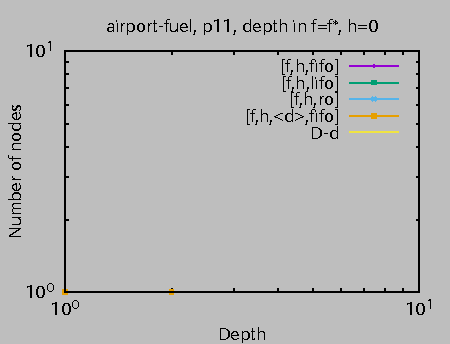
\includegraphics{img/depth/airport-fuel/p11.pdf}
% 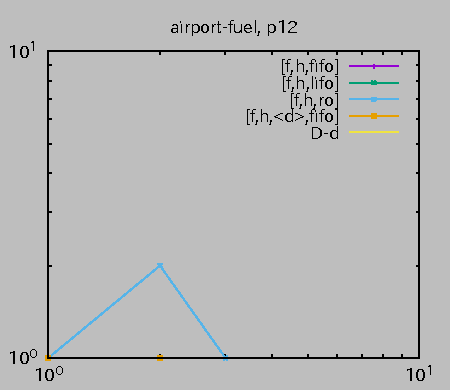
\includegraphics{img/depth/airport-fuel/p12.pdf}
% 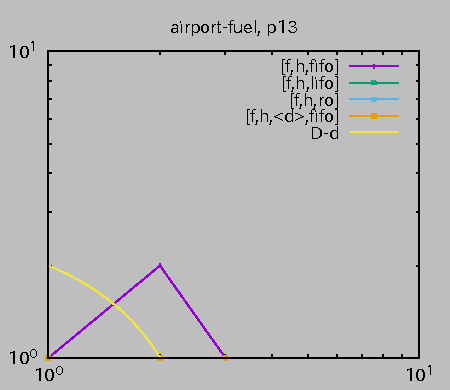
\includegraphics{img/depth/airport-fuel/p13.pdf}
% 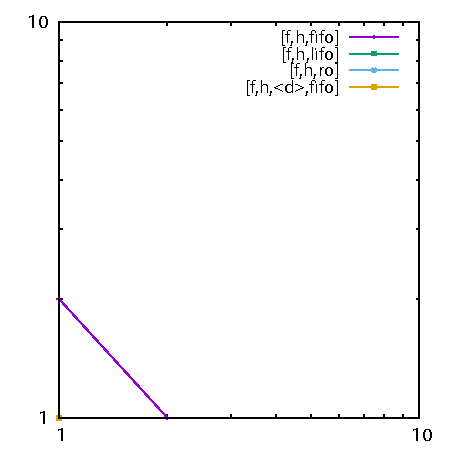
\includegraphics{img/depth/airport-fuel/p14.pdf}
% 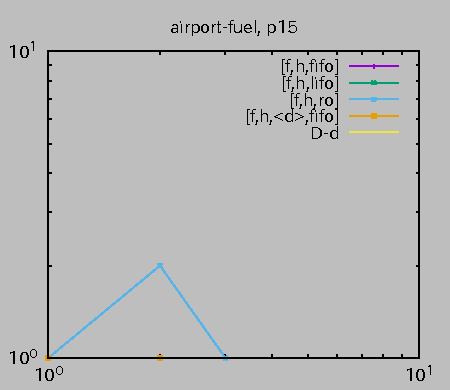
\includegraphics{img/depth/airport-fuel/p15.pdf}
% 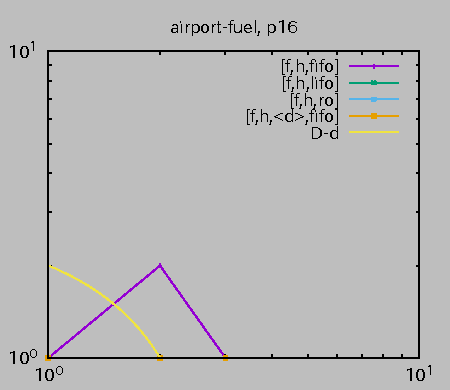
\includegraphics{img/depth/airport-fuel/p16.pdf}
% 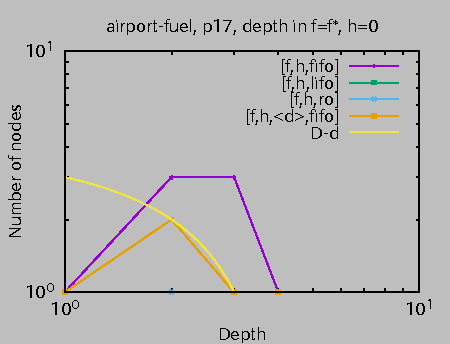
\includegraphics{img/depth/airport-fuel/p17.pdf}
% 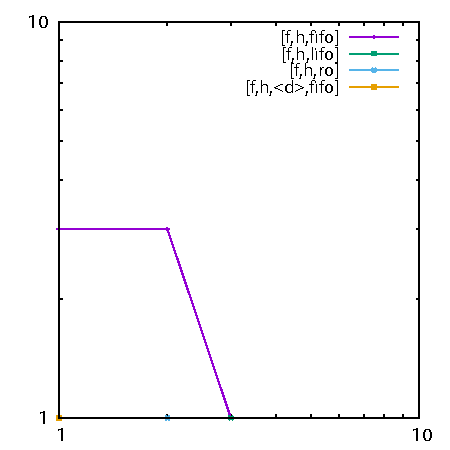
\includegraphics{img/depth/airport-fuel/p18.pdf}
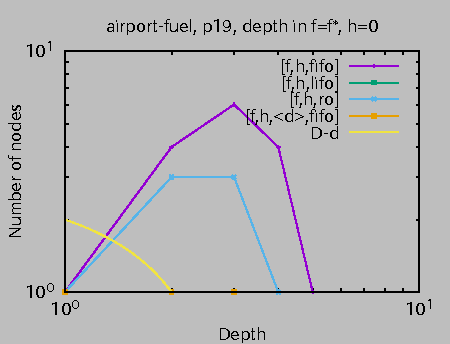
\includegraphics{img/depth/airport-fuel/p19.pdf}
% 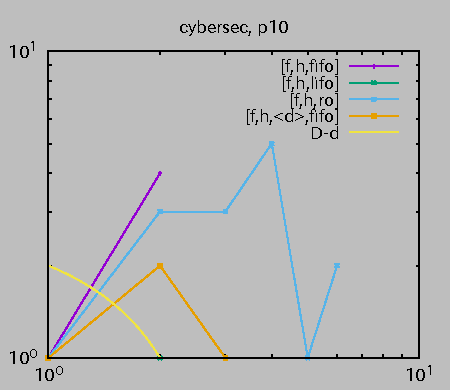
\includegraphics{img/depth/cybersec/p10.pdf}
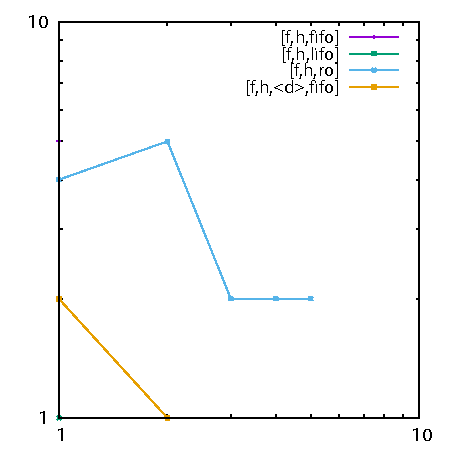
\includegraphics{img/depth/cybersec/p11.pdf}
% 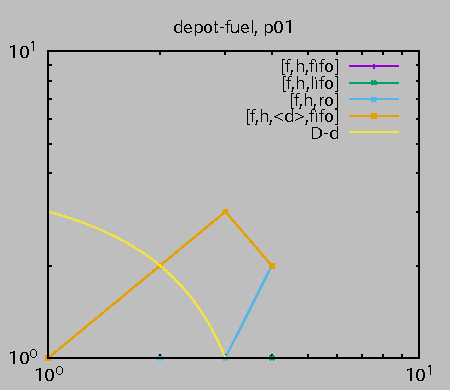
\includegraphics{img/depth/depot-fuel/p01.pdf}
% 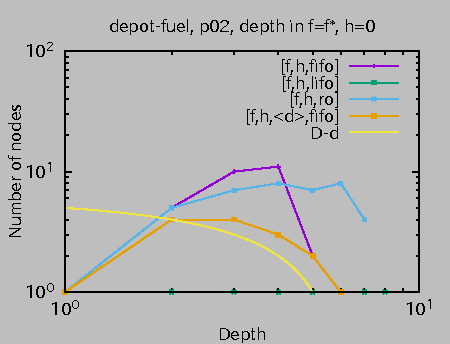
\includegraphics{img/depth/depot-fuel/p02.pdf}
% 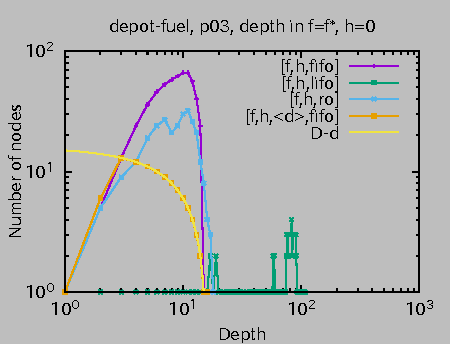
\includegraphics{img/depth/depot-fuel/p03.pdf}
% 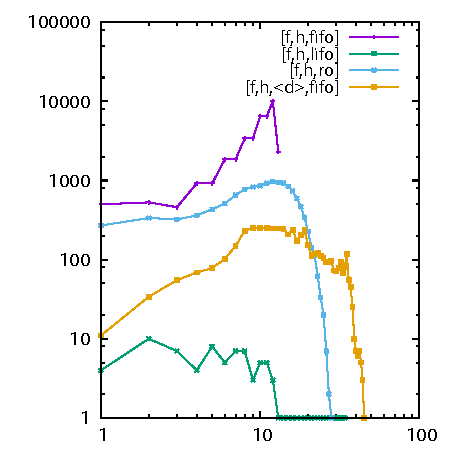
\includegraphics{img/depth/depot-fuel/p04.pdf}
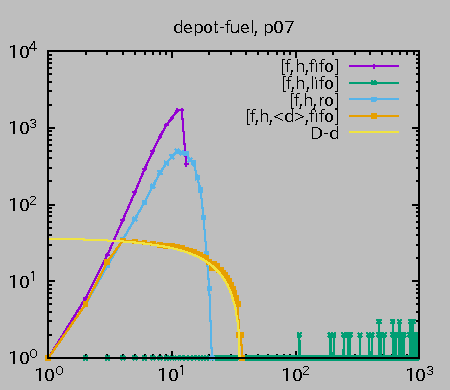
\includegraphics{img/depth/depot-fuel/p07.pdf}
% 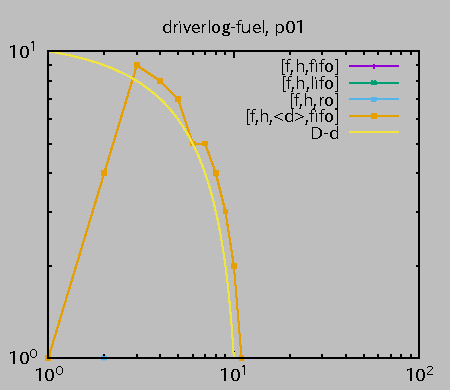
\includegraphics{img/depth/driverlog-fuel/p01.pdf}
% 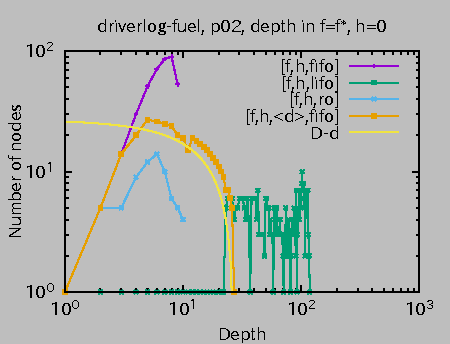
\includegraphics{img/depth/driverlog-fuel/p02.pdf}
% 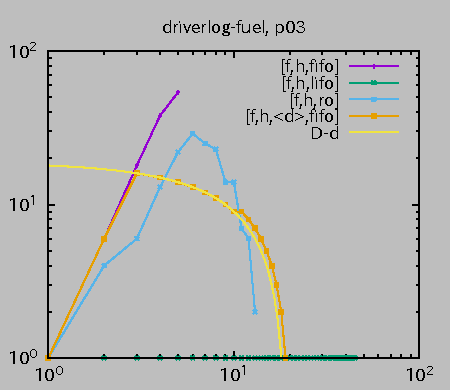
\includegraphics{img/depth/driverlog-fuel/p03.pdf}
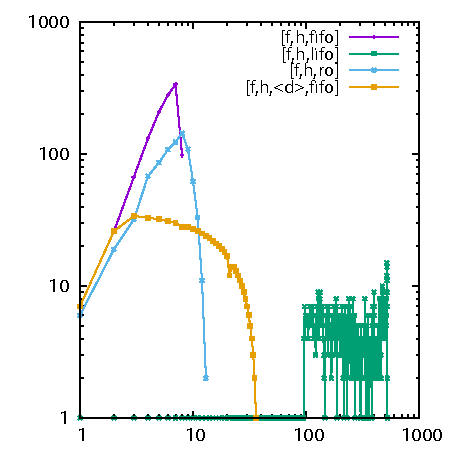
\includegraphics{img/depth/driverlog-fuel/p04.pdf}
% 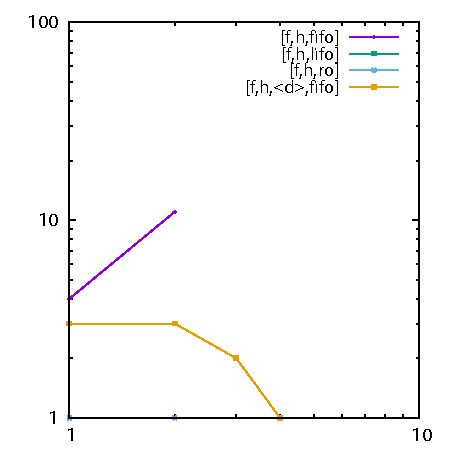
\includegraphics{img/depth/driverlog-fuel/p05.pdf}
% 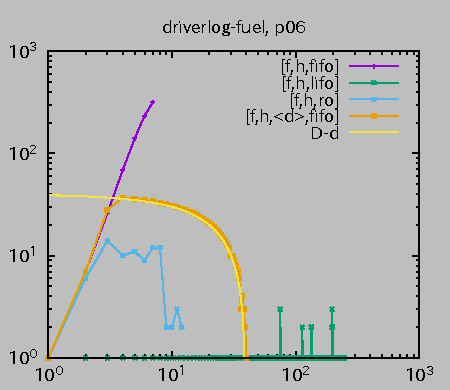
\includegraphics{img/depth/driverlog-fuel/p06.pdf}
% 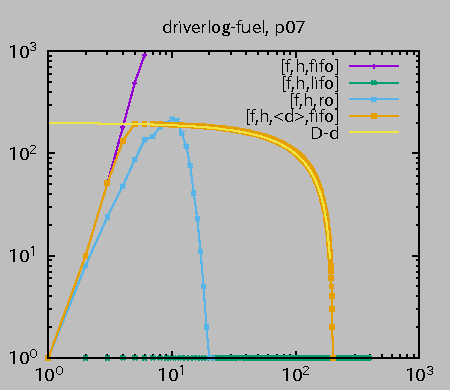
\includegraphics{img/depth/driverlog-fuel/p07.pdf}
% 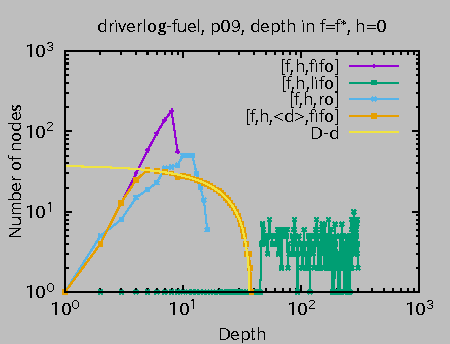
\includegraphics{img/depth/driverlog-fuel/p09.pdf}
% 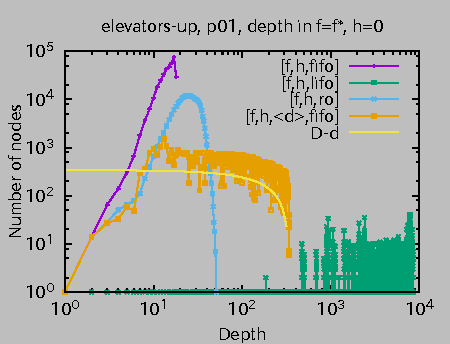
\includegraphics{img/depth/elevators-up/p01.pdf}
% 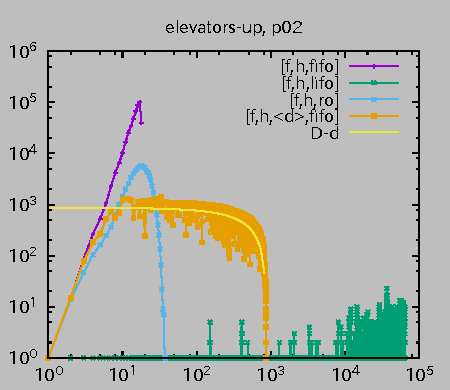
\includegraphics{img/depth/elevators-up/p02.pdf}
% 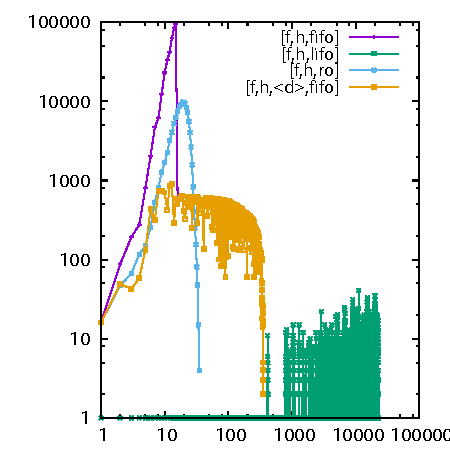
\includegraphics{img/depth/elevators-up/p03.pdf}
% 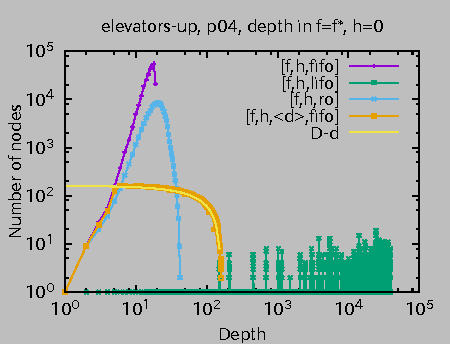
\includegraphics{img/depth/elevators-up/p04.pdf}
% 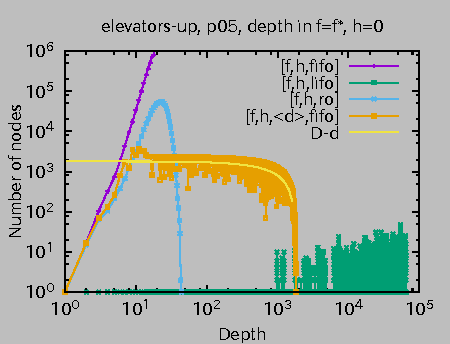
\includegraphics{img/depth/elevators-up/p05.pdf}
% 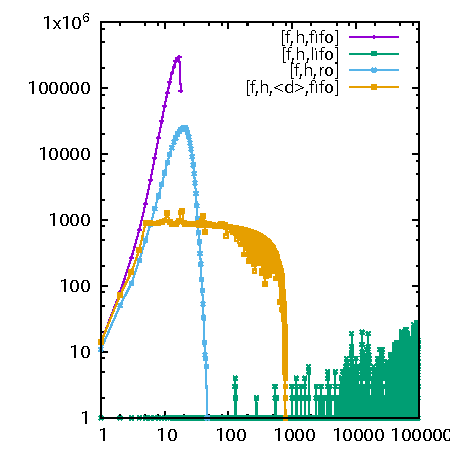
\includegraphics{img/depth/elevators-up/p06.pdf}
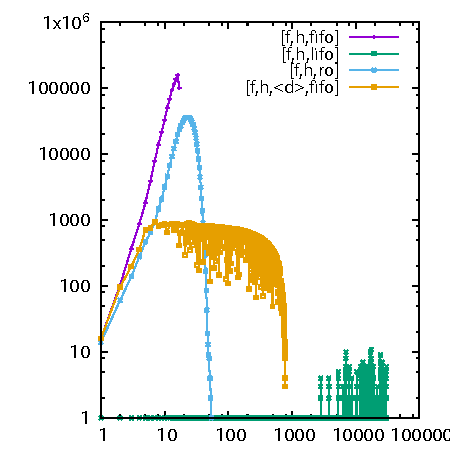
\includegraphics{img/depth/elevators-up/p09.pdf}
% 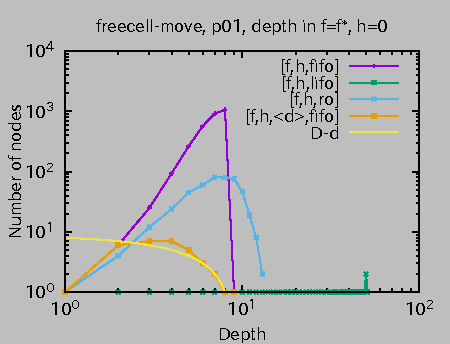
\includegraphics{img/depth/freecell-move/p01.pdf}
% 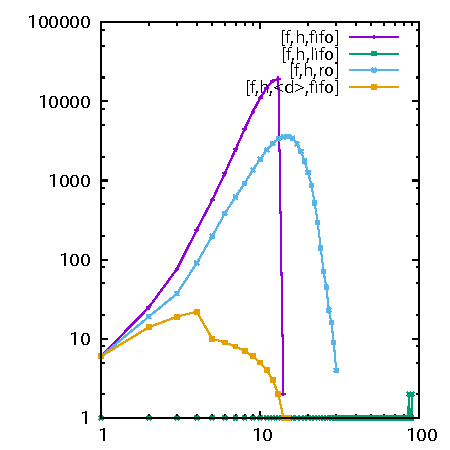
\includegraphics{img/depth/freecell-move/p02.pdf}
% 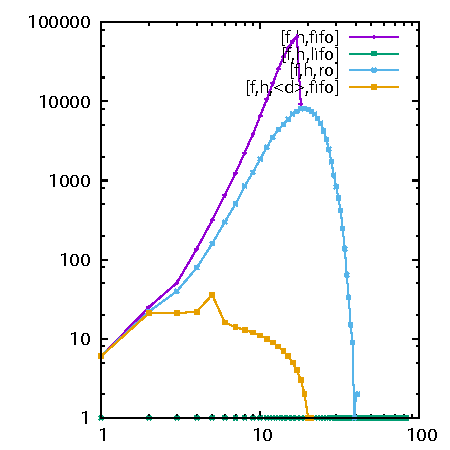
\includegraphics{img/depth/freecell-move/p03.pdf}
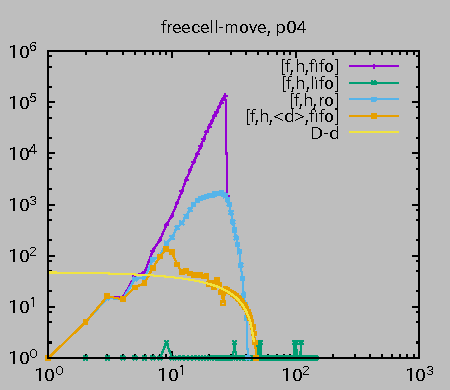
\includegraphics{img/depth/freecell-move/p04.pdf}
% 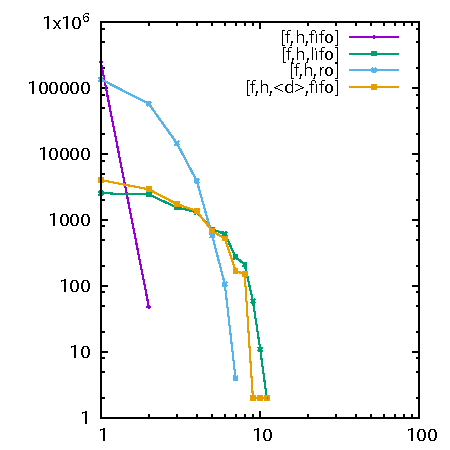
\includegraphics{img/depth/ged-opt14-strips/p11.pdf}
% 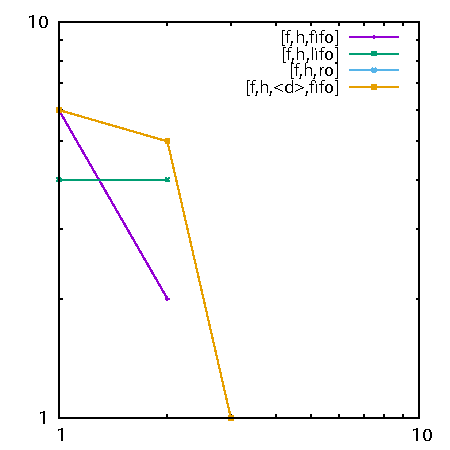
\includegraphics{img/depth/ged-opt14-strips/p12.pdf}
% 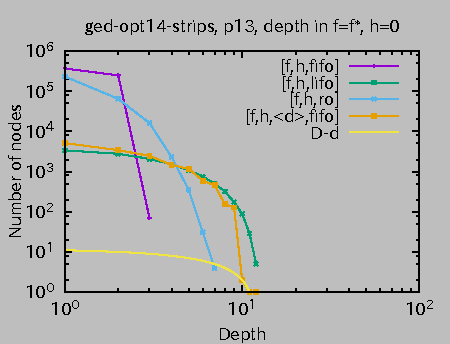
\includegraphics{img/depth/ged-opt14-strips/p13.pdf}
% 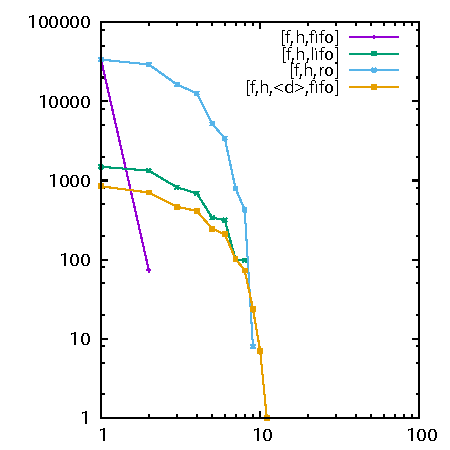
\includegraphics{img/depth/ged-opt14-strips/p15.pdf}
% 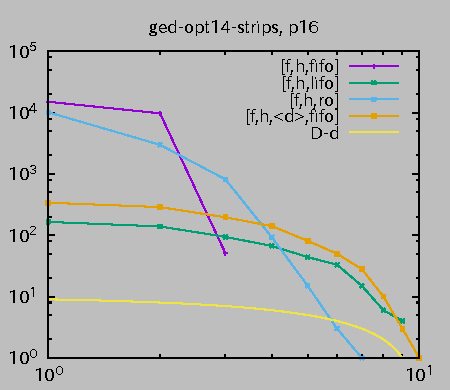
\includegraphics{img/depth/ged-opt14-strips/p16.pdf}
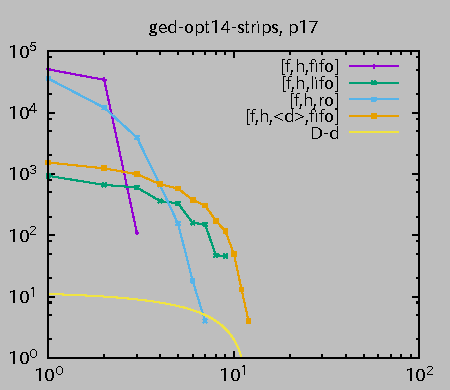
\includegraphics{img/depth/ged-opt14-strips/p17.pdf}
% 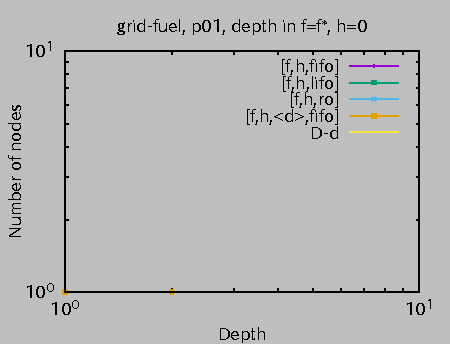
\includegraphics{img/depth/grid-fuel/p01.pdf}
% 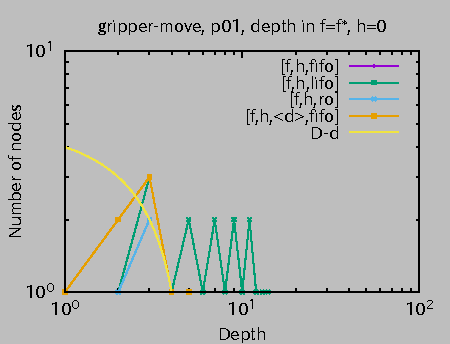
\includegraphics{img/depth/gripper-move/p01.pdf}
% 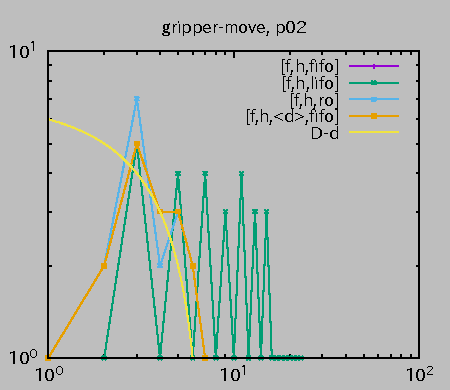
\includegraphics{img/depth/gripper-move/p02.pdf}
% 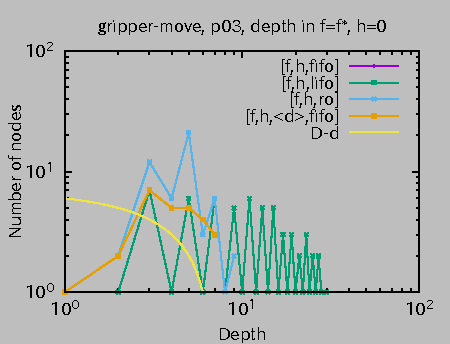
\includegraphics{img/depth/gripper-move/p03.pdf}
% 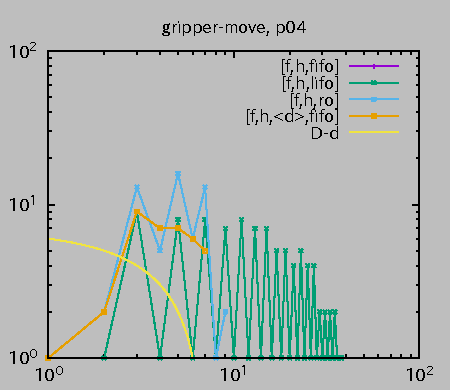
\includegraphics{img/depth/gripper-move/p04.pdf}
% 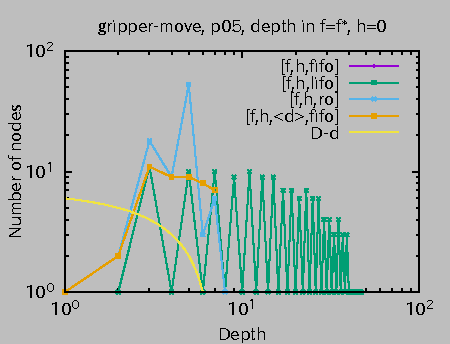
\includegraphics{img/depth/gripper-move/p05.pdf}
% 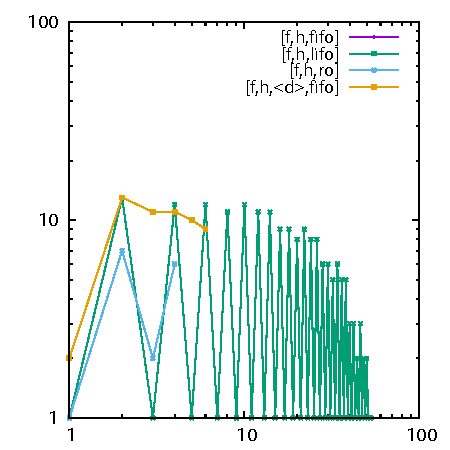
\includegraphics{img/depth/gripper-move/p06.pdf}
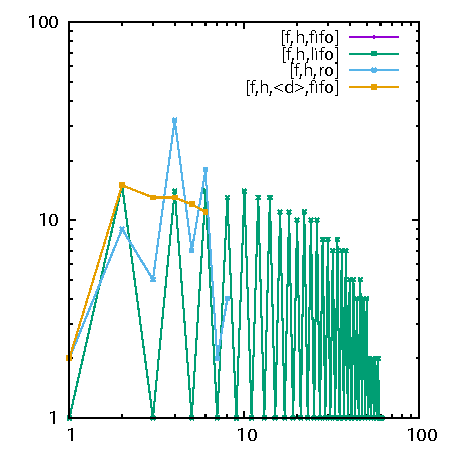
\includegraphics{img/depth/gripper-move/p07.pdf}
% 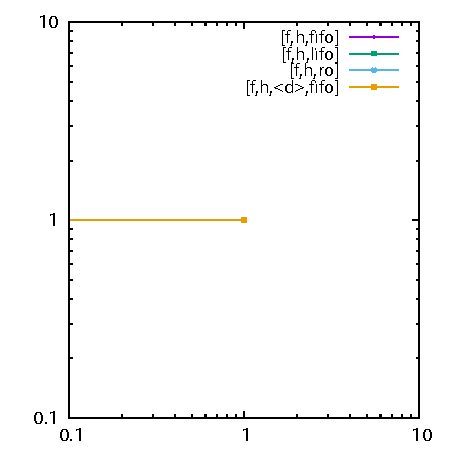
\includegraphics{img/depth/hiking-fuel/p01.pdf}
% \includegraphics{img/depth/hiking-fuel/p02.pdf}
% \includegraphics{img/depth/hiking-fuel/p03.pdf}
% \includegraphics{img/depth/hiking-fuel/p04.pdf}
% \includegraphics{img/depth/hiking-fuel/p05.pdf}
% \includegraphics{img/depth/hiking-fuel/p06.pdf}
% \includegraphics{img/depth/hiking-fuel/p07.pdf}
% \includegraphics{img/depth/logistics00-fuel/p010.pdf}
% \includegraphics{img/depth/logistics00-fuel/p011.pdf}
% \includegraphics{img/depth/logistics00-fuel/p012.pdf}
% \includegraphics{img/depth/logistics00-fuel/p013.pdf}
% \includegraphics{img/depth/logistics00-fuel/p014.pdf}
% \includegraphics{img/depth/logistics00-fuel/p015.pdf}
\includegraphics{img/depth/logistics00-fuel/p016.pdf}
% \includegraphics{img/depth/logistics00-fuel/p017.pdf}
% \includegraphics{img/depth/miconic-up/p59.pdf}
% \includegraphics{img/depth/miconic-up/p63.pdf}
% \includegraphics{img/depth/miconic-up/p67.pdf}
% \includegraphics{img/depth/miconic-up/p75.pdf}
\includegraphics{img/depth/miconic-up/p79.pdf}
% \includegraphics{img/depth/mystery-feast/p01.pdf}
% \includegraphics{img/depth/mystery-feast/p03.pdf}
% \includegraphics{img/depth/mystery-feast/p09.pdf}
% \includegraphics{img/depth/nomystery-fuel/p01.pdf}
% \includegraphics{img/depth/nomystery-fuel/p02.pdf}
% \includegraphics{img/depth/nomystery-fuel/p03.pdf}
% \includegraphics{img/depth/nomystery-fuel/p04.pdf}
% \includegraphics{img/depth/nomystery-fuel/p05.pdf}
% \includegraphics{img/depth/openstacks-opt11-strips/p06.pdf}
\includegraphics{img/depth/openstacks-opt11-strips/p07.pdf}
% \includegraphics{img/depth/openstacks-opt11-strips/p08.pdf}
% \includegraphics{img/depth/openstacks-opt11-strips/p09.pdf}
% \includegraphics{img/depth/openstacks-opt11-strips/p10.pdf}
% \includegraphics{img/depth/pathways-fuel/p01.pdf}
% \includegraphics{img/depth/pathways-fuel/p02.pdf}
\includegraphics{img/depth/pathways-fuel/p03.pdf}
% \includegraphics{img/depth/pathways-fuel/p04.pdf}
\includegraphics{img/depth/pipesnt-pushstart/p06.pdf}
% \includegraphics{img/depth/pipesnt-pushstart/p07.pdf}
% \includegraphics{img/depth/pipesnt-pushstart/p08.pdf}
% \includegraphics{img/depth/pipesnt-pushstart/p11.pdf}
% \includegraphics{img/depth/pipesnt-pushstart/p13.pdf}
\includegraphics{img/depth/pipesworld-pushend/p06.pdf}
% \includegraphics{img/depth/pipesworld-pushend/p15.pdf}
% \includegraphics{img/depth/psr-small-open/p42.pdf}
% \includegraphics{img/depth/psr-small-open/p43.pdf}
% \includegraphics{img/depth/psr-small-open/p44.pdf}
% \includegraphics{img/depth/psr-small-open/p45.pdf}
\includegraphics{img/depth/psr-small-open/p46.pdf}
% \includegraphics{img/depth/psr-small-open/p47.pdf}
% \includegraphics{img/depth/psr-small-open/p48.pdf}
% \includegraphics{img/depth/psr-small-open/p50.pdf}
% \includegraphics{img/depth/rovers-fuel/p01.pdf}
% \includegraphics{img/depth/rovers-fuel/p02.pdf}
% \includegraphics{img/depth/rovers-fuel/p03.pdf}
% \includegraphics{img/depth/rovers-fuel/p04.pdf}
% \includegraphics{img/depth/rovers-fuel/p05.pdf}
% \includegraphics{img/depth/rovers-fuel/p06.pdf}
\includegraphics{img/depth/rovers-fuel/p07.pdf}
% \includegraphics{img/depth/scanalyzer-analyze/p01.pdf}
% \includegraphics{img/depth/scanalyzer-analyze/p02.pdf}
% \includegraphics{img/depth/scanalyzer-analyze/p03.pdf}
\includegraphics{img/depth/scanalyzer-analyze/p04.pdf}
% \includegraphics{img/depth/scanalyzer-analyze/p06.pdf}
\includegraphics{img/depth/storage-lift/p11.pdf}
% \includegraphics{img/depth/storage-lift/p12.pdf}
% \includegraphics{img/depth/storage-lift/p13.pdf}
% \includegraphics{img/depth/storage-lift/p14.pdf}
% \includegraphics{img/depth/tidybot-motion/p06.pdf}
% \includegraphics{img/depth/tidybot-motion/p07.pdf}
% \includegraphics{img/depth/tidybot-motion/p08.pdf}
% \includegraphics{img/depth/tidybot-motion/p09.pdf}
% \includegraphics{img/depth/tidybot-motion/p10.pdf}
% \includegraphics{img/depth/tidybot-motion/p11.pdf}
% \includegraphics{img/depth/tidybot-motion/p12.pdf}
% \includegraphics{img/depth/tidybot-motion/p13.pdf}
% \includegraphics{img/depth/tidybot-motion/p14.pdf}
\includegraphics{img/depth/tidybot-motion/p16.pdf}
% \includegraphics{img/depth/tpp-fuel/p01.pdf}
% \includegraphics{img/depth/tpp-fuel/p02.pdf}
% \includegraphics{img/depth/tpp-fuel/p03.pdf}
% \includegraphics{img/depth/tpp-fuel/p04.pdf}
% \includegraphics{img/depth/tpp-fuel/p05.pdf}
% \includegraphics{img/depth/tpp-fuel/p06.pdf}
% \includegraphics{img/depth/tpp-fuel/p07.pdf}
\includegraphics{img/depth/tpp-fuel/p08.pdf}
% \includegraphics{img/depth/woodworking-cut/p01.pdf}
% \includegraphics{img/depth/woodworking-cut/p02.pdf}
% \includegraphics{img/depth/woodworking-cut/p03.pdf}
\includegraphics{img/depth/woodworking-cut/p04.pdf}
% \includegraphics{img/depth/woodworking-cut/p07.pdf}
% \includegraphics{img/depth/zenotravel-fuel/p02.pdf}
% \includegraphics{img/depth/zenotravel-fuel/p03.pdf}
% \includegraphics{img/depth/zenotravel-fuel/p04.pdf}
% \includegraphics{img/depth/zenotravel-fuel/p05.pdf}
% \includegraphics{img/depth/zenotravel-fuel/p06.pdf}
\includegraphics{img/depth/zenotravel-fuel/p07.pdf} % \centering \relsize{-3}
 % \hfill
 % \includegraphics{tables/aaai16-log-rd/aaai16prelim3/depth-histogram-openstacks-opt11-strips-p10.pdf}
 % \hfill
 % \includegraphics{tables/aaai16-log-rd/2zerocost/depth-histogram-woodworking-cut-p04.pdf}
 % \hfill
 % \includegraphics{tables/aaai16-log-rd/2zerocost/depth-histogram-psr-small-open-p48.pdf}
 \caption{Number of nodes ($y$-axis) expanded per depth ($x$-axis) in
 the final plateau with different tiebreakings. Both axes are in logarithmic scale.
 }
 \label{fig:depth-histogram}
\end{figure}

% airport-fuel/	 ged-opt14-strips/  nomystery-fuel/	      sokoban-pushgoal/
% blocks-stack/	 grid-fuel/	    openstacks-opt11-strips/  storage-lift/
% cybersec/	 gripper-move/	    pathways-fuel/	      tidybot-motion/
% depot-fuel/	 hiking-fuel/	    pipesnt-pushstart/	      tpp-fuel/
% driverlog-fuel/  logistics00-fuel/  pipesworld-pushend/       woodworking-cut/
% elevators-up/	 miconic-up/	    psr-small-open/	      zenotravel-fuel/
% floortile-ink/	 mprime-succumb/    rovers-fuel/
% freecell-move/	 mystery-feast/     scanalyzer-analyze/



\subsection{Comparison to Distance-to-Go Estimates}

We next compare our depth diversification to the distance-to-go
estimates in the plateau.  Distance-to-go estimates are the type of
heuristics which treat actions as if they have the unit cost. Even under
the presence of zero-cost actions, those estimates can predict the
number of operations required to reach a goal.

While several papers advocates the benefit of this technique, many of
these claims took place in the context of satisficing planning.
\cite{benton2010g} proposes inadmissible technique for temporal planning
where short actions are hidden behind long actions and do not increase makespan.
They implemented an inadmissible heuristic function on top of Temporal Fast
Downward system and evaluated it on \astar.
As stated, their method is not applicable to the optimising search.
Similarly, \cite{cushing2010cost,wilt2011cost} showed that (non-admissibly) treating all
actions as unit cost sometimes finds an optimal plan quickly. Although
it could find an optimal plan by chance, this does not guarantee the
optimality of the solution.

Still, there is a number of possibilities to adopt the idea of
distance-to-go in optimal search. One such example is to use the
distance-to-go estimates as part of sorting criteria.
% 
Let $\hat{h}$ be a variation of original heuristic function
$h$. $\hat{h}$ computes the distance-to-go estimates by treating all
actions to be unit cost, while original heuristic function $h$ uses the
standard action cost to compute the value.

Now, as long as the first sorting criteria is based on $f=g+h$, any
sorting strategy returns an optimal solution. Thus, it is possible to
use a multi-heuristic strategy such as $[f,h,\hat{h}]$ or $[f,\hat{h}]$
which uses inadmissible $\hat{h}$ as part of sorting criteria.
In fact, it is even possible to use any inadmissible heuristic function to break
ties. For example, one can use inadmissible FF heuristics to break ties
among $f$ which uses admissible \lmcut heuristic function -- $[h^{\lmcut}+g,\hat{h}^{\ff}]$.

There are number of possible combinations here, but the obvious flaw in
such a strategy is the cost of computing additional heuristic
estimates. Using different heuristics obviously causes such an
overhead. Using distance-to-go estimates $\hat{h}$ along with original
heuristics $h$ could be optimized so that it shares part of the
computation, but still should incur some overhead.

We tested various combinations of heuristics on zerocost domains where
tiebreaking strategies have the large impact.
We tested the following configurations:
$[h^{\lmcut}+g,h^{\lmcut},\fifo]$, 
$[h^{\lmcut}+g,h^{\lmcut},\depth,\fifo]$, 
$[h^{\lmcut}+g,h^{\lmcut},\hat{h}^{\lmcut},\fifo]$, 
$[h^{\lmcut}+g,\hat{h}^{\lmcut},\fifo]$, 
$[h^{\lmcut}+g,\hat{h}^{\ff},\fifo]$,
$[h^{\lmcut}+g,\hat{h}^{\mbox{GC}},\fifo]$.

% $[h^{\lmcut}+g,\hat{h}^{\mbox{LMcount}},\fifo]$,
